\clearpage
\pagenumbering{arabic}
\setcounter{page}{1}

\phantomsection
\label{ch:intro}
\chapter{Introduction}

This chapter presents the main components of this research on Khmer optical character recognition (OCR). It begins with background information on OCR technology and its importance for the Khmer language, followed by identifying the key challenges and research gaps in current Khmer OCR systems. The chapter then outlines the study's objectives and research questions focused on improving Khmer text recognition through synthetic data generation and deep learning approaches. The rationale highlights the significance of developing better OCR tools for preserving and digitizing Khmer texts. Finally, it describes the scope and limitations of the study, along with an overview of the thesis structure.

\section{Background to the Study}
\label{sec:background}

In recent decades, Optical Character Recognition (OCR) technology—powered by advancements in Artificial Intelligence (AI)—has revolutionized the way physical texts are converted into machine-readable formats. AI-based OCR systems use deep learning models to detect, segment, and classify characters from images or scanned documents, enabling efficient digitization of printed or handwritten text. These systems form a critical foundation for applications in digital libraries, information retrieval, natural language processing, and AI-powered search systems.

Globally, OCR for high-resource languages such as English, Chinese, and Japanese has been extensively researched and developed over the last eight decades \citep{memon2020handwritten}. These systems benefit from large annotated datasets, robust typographic models, and standardized script structures. In contrast, OCR development for low-resource languages like Khmer remains significantly underdeveloped.

In Cambodia, OCR technology has become increasingly important due to the growing demand for digitized content across sectors such as education and research. The past two decades have seen rapid growth in digital adoption, resulting in a pressing need for intelligent systems capable of processing Khmer-language documents efficiently.

Khmer is the official language of the Kingdom of Cambodia and is also used to write other minority languages such as Kuay, Tampuan, Jarai, Krung, Brao, and Kravet. The Khmer writing system, which dates back to the 7th century, is an abugida script featuring complex combinations of consonants, subscript forms, diacritics, and vowel markers. Unlike Latin-based scripts, Khmer characters can stack vertically or combine in ways that affect the spatial layout and visual appearance of the text. As a result, OCR for Khmer requires not only accurate character recognition but also careful handling of contextual dependencies between character components.

A complete Khmer OCR system must be capable of recognizing all script elements. Any omission—such as failing to detect a subscript or diacritic—can lead to incorrect rendering or interpretation of the entire word. Due to this complex layout rendering, character-level accuracy is critical for preserving the meaning and readability of digitized Khmer texts.

The growing need for Khmer OCR technology is particularly evident in the education sector. Many school textbooks from grade 1 to 12 exist only in physical form, with no digital versions available due to the loss or absence of original files. This severely limits accessibility and updatability in modern digital learning environments. Table~\ref{sec:textbook} summarizes the current state of Khmer textbook digitization.


\begin{table}[ht]
    \caption{Current State of Khmer Textbook Digitization in Cambodia's Education System}
    \vspace{10pt}
    \phantomsection
    \label{sec:textbook}
    \resizebox{\textwidth}{!}{
    \begin{tabular}{|l|l|l|l|}
    \hline
    Education Level & Subject Areas & Format Availability & Notes \\
    \hline
    Grade 1--6 & All core subjects & Mostly physical only & Many original digital files missing \\
    Grade 7--9 & Math, Science, Khmer & Some digital scans & Scanned PDFs, not text-searchable \\
    Grade 10--12 & All major subjects & Few digitized & Hard to find editable versions \\
    \hline
    \end{tabular}
    }
\end{table}

Beyond education, Khmer OCR has broader implications across multiple sectors:

\begin{itemize}
    \item \textbf{Digital Libraries:} Converting physical Khmer books into searchable formats enables efficient access to national knowledge repositories.
    
    \item \textbf{Cultural Heritage:} Ancient palm leaf manuscripts and religious texts can be preserved digitally and accessed by scholars and AI systems.
    
    \item \textbf{Government Records:} Legal, civil, and administrative documents can be digitized for automated search, archiving, and public service use.
    
    \item \textbf{Healthcare:} Khmer OCR can support the digitization of medical records, improving data accessibility and enabling medical AI models.
    
    \item \textbf{AI and NLP Applications:} Digitized Khmer texts can be used to train AI language models, making systems more inclusive and capable of understanding Khmer input.
    
    \item \textbf{Business Intelligence:} Companies can extract structured data from scanned Khmer documents for analytics and automation.
    
    \item \textbf{Media Archives:} Historical newspapers and magazines can be processed for research into social, political, and cultural trends.
\end{itemize}

In summary, OCR technology in Cambodia is no longer a niche research area but a national priority aligned with the country’s digital transformation roadmap. With Khmer script presenting significant challenges and opportunities, developing a robust OCR system is essential for Cambodia’s progress toward a digital future.



\section{Problem Statement}
\label{sec:problem}

Optical Character Recognition (OCR) for the Khmer language presents a 
unique set of challenges that significantly hinder the development 
of accurate and robust recognition systems. Unlike Latin-based scripts, 
Khmer is an abugida writing system, where each character represents a 
consonant-vowel unit and includes complex combinations of base 
characters, subscripts, superscripts, and diacritics. This structural 
complexity introduces difficulties at both the text detection 
stage and the text recognition stage.
\begin{figure}[ht]
    \centering
    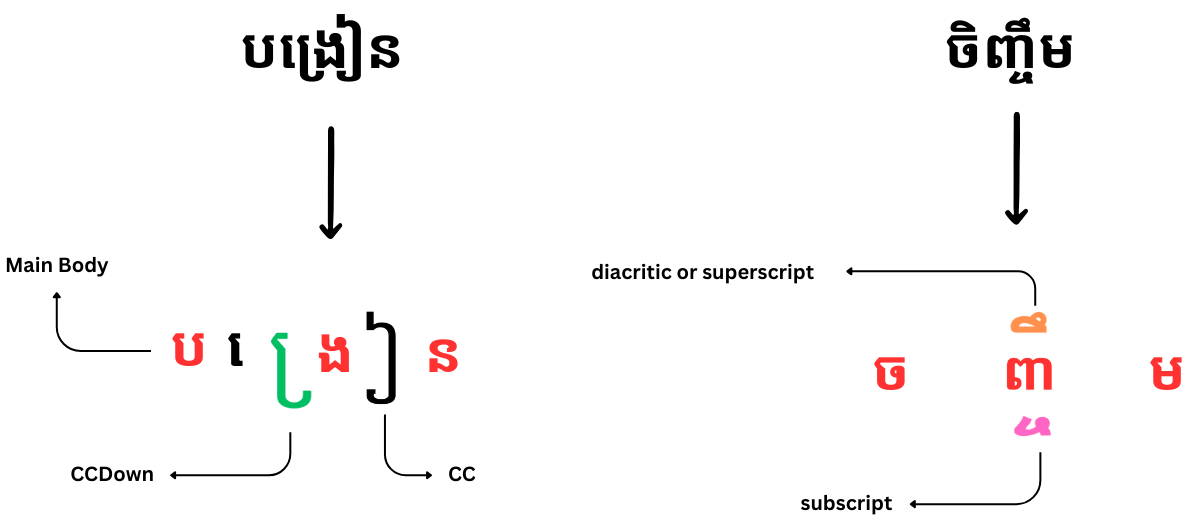
\includegraphics[width=\textwidth]{figures/example_of_text_format.png}
    \caption{Example of Khmer text format showing the complexity of character combinations and diacritics}
    \label{fig:text_format}
\end{figure}

One of the fundamental obstacles is the lack of clear word boundaries 
in Khmer writing. In contrast to Latin-based languages, 
where spaces are consistently used to separate words, 
spaces in Khmer are used infrequently and inconsistently. 
This makes it extremely difficult to segment text accurately 
into word-level units for training sequence-to-sequence OCR models 
such as TrOCR. The absence of reliable word boundaries reduces 
recognition accuracy and complicates tasks like error correction, 
search indexing, and language modeling.

\begin{figure}[ht]
    \centering
    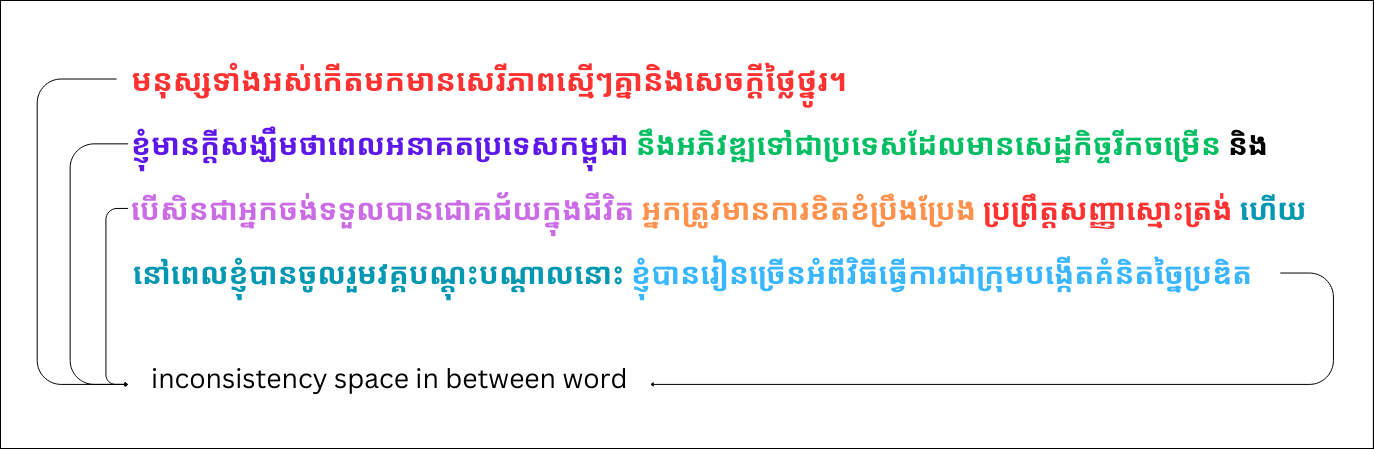
\includegraphics[width=\textwidth]{figures/example_of_long_text.png}
    \caption{Example of sequential Khmer text showing how characters combine to form syllables and words}
    \label{fig:sequential_text}
\end{figure}


A critical barrier to advancing Khmer OCR is the scarcity of annotated training datasets. There is a severe lack of high-quality, large-scale datasets that provide paired image-text data with bounding boxes, character-level annotations, or transcription lines tailored to Khmer script. This data scarcity limits the potential for supervised learning approaches and transfer learning, which are essential for training modern deep OCR models like TrOCR.


Additionally, font and style variability further degrade recognition performance. Khmer documents in the real world are printed in diverse typefaces and stylistic variations (e.g., Khmer OS, Nokora, and Hanuman), with differences in stroke thickness, spacing, and decoration. The lack of standardization across documents and poor documentation of these fonts means that OCR models trained on one style often fail to generalize to others. This problem is exacerbated in noisy or low-resolution scans of textbooks and historical texts.

The challenge of font variability is illustrated in Figure \ref{fig:font_variants}, which shows how the same Khmer text can appear significantly different across various fonts and styles.

\begin{figure}[ht]
    \centering
    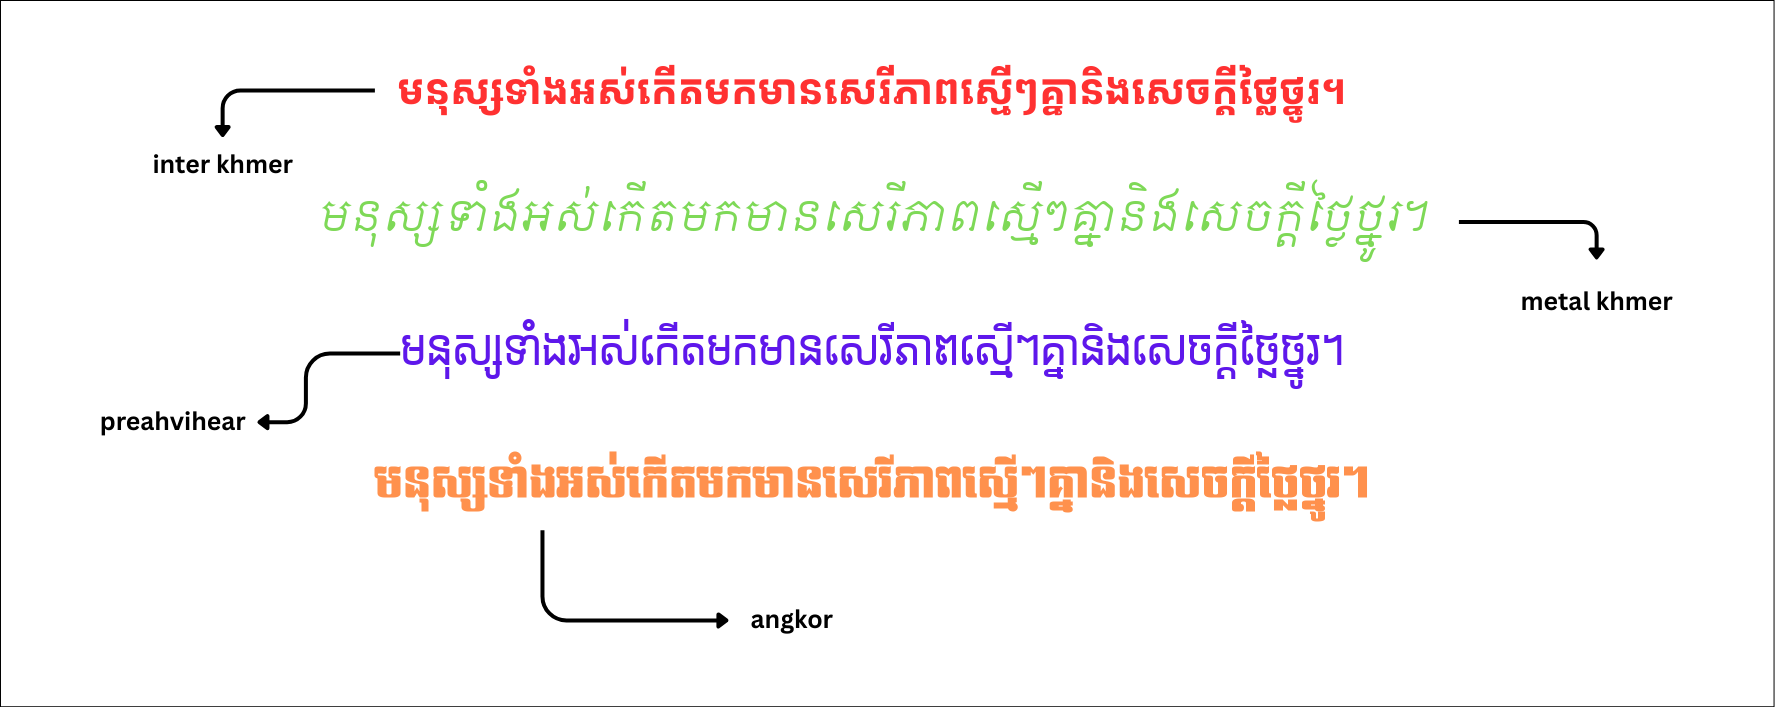
\includegraphics[width=\textwidth]{figures/varianty_of_font.png}
    \caption{Examples of the same Khmer text rendered in different fonts, demonstrating the significant visual variations that OCR systems must handle}
    \label{fig:font_variants}
\end{figure}

\begin{figure}[ht]
    \centering
    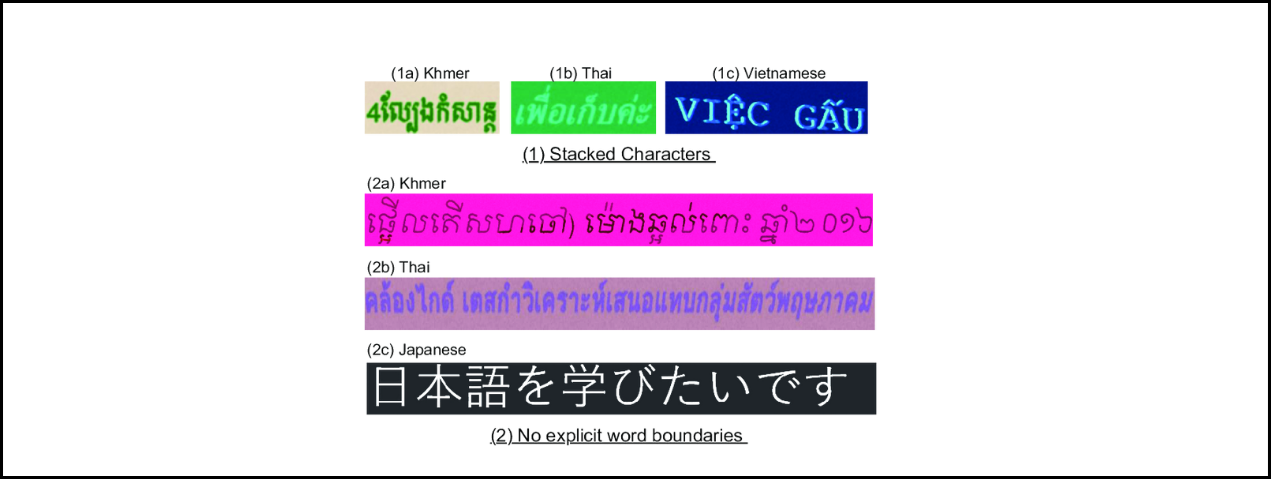
\includegraphics[width=\textwidth]{figures/text_stacking_mixing_language.png}
    \caption{Illustration of Khmer text stacking patterns, 
    showing how characters combine vertically and horizontally 
    to form syllables and words \citep{buoy2023khmerocr}}
    \label{fig:text_stacking}
\end{figure}

Taken together, these challenges create a significant barrier to digitizing Khmer documents using CRAFT + TrOCR pipelines. The absence of word delimiters, the visual complexity of character stacking, cross-script confusion, data scarcity, and font inconsistency all contribute to the low accuracy and poor reliability of existing OCR solutions for Khmer. Addressing these issues requires the development of customized preprocessing, augmentation, and model training strategies—as well as targeted data collection and annotation efforts—to make Khmer OCR viable for real-world applications, especially in the context of educational digitization and cultural preservation.




\section{Aim and Objectives of the Study}
\label{sec:objectives}

The primary aim of this research is to develop an improved optical character recognition (OCR) system specifically designed for MIX-language (Khmer-English) addressing the unique challenges of Khmer-English script while achieving high accuracy and reliability in real-world applications.

The specific objectives of this study are:

\begin{enumerate}
    \item To create text annotation tool to bounding boxes for create real-dataset for Khmer-English for both text detection and text recognition tasks.
    \item To create a robust training dataset such as varianty of font, real-world environment that addresses the lack of annotated data for Khmer OCR
    \item To develop end-to-end OCR pipelines such as text detection and recognition models that utilizing CRAFT and TrOCR model architectures, particularly focusing on text line based segmentation.
    \item To achieve the state-of-the-art (Accuracy \& CER) and reliability in real-world applications for Khmer-English OCR.
\end{enumerate}

Through achieving these objectives, this research aims to significantly advance the state of Khmer OCR technology and enable more effective digitization of Cambodian textual heritage.

\section{Research Questions}
\label{sec:questions}

This research aims to address the following key questions:

\begin{enumerate}
    \item How can text detection and recognition models be effectively adapted to handle the unique characteristics of Khmer script, particularly the stacking of characters and presence of diacritics?
    
    \item What preprocessing and augmentation techniques are most effective for improving OCR accuracy on Khmer text documents with varying fonts, styles, and quality levels?

    \item What are the minimum dataset requirements and optimal annotation strategies for training robust Khmer OCR models?
    
    \item What is the whole pipeline used to convert document image into digital text on Khmer script with the most Effectiveness?
\end{enumerate}

\section{Rationale of the Study}
\label{sec:rationale}
       This research is motivated by several compelling factors. First, there is an urgent need to digitize and preserve Cambodia's vast textual heritage, including historical documents, educational materials, and cultural artifacts. Without effective OCR technology for Khmer script, this digitization process remains labor-intensive and prone to errors.

Second, the current limitations of OCR systems for Khmer significantly hinder educational and academic initiatives in Cambodia. Many educational institutions struggle to convert physical textbooks and learning materials into digital formats, impacting accessibility and modernization efforts in education.

Third, the unique challenges posed by Khmer script—from character stacking to the absence of word boundaries—present an opportunity to advance the field of OCR technology as a whole. Solutions developed for Khmer may benefit other scripts with similar characteristics.

Finally, improving Khmer OCR technology aligns with broader digital transformation goals in Cambodia, supporting efforts to preserve cultural heritage while enabling more efficient information processing and accessibility in various sectors.

\section{Limitations and Scope}
\label{sec:limitations}

While this research aims to advance Khmer OCR technology significantly, it is important to acknowledge certain limitations and define the scope of the study:

\begin{enumerate}
    \item The research focuses specifically on printed Khmer text and English text and does not address handwritten text recognition, which presents additional challenges requiring separate investigation.
    
    \item The study primarily considers modern Khmer fonts and typography, with limited coverage of historical or decorative text styles.
    
    \item While the system aims to handle various document quality levels, extremely degraded or damaged documents may fall outside the scope of reliable recognition.
    
    \item The study focuses on optical character recognition and does not extend to higher-level natural language processing tasks such as semantic analysis or machine translation.
    
    \item Resource constraints may limit the size and diversity of the training dataset, though efforts will be made to ensure sufficient representation of common use cases.
\end{enumerate}

These limitations help maintain a focused research scope while acknowledging areas that may require future investigation.

\section{Structure of the Thesis}
\label{sec:structure}

This thesis is organized into the following chapters:

\begin{enumerate}
    \item \textbf{Introduction}: Presents the research background, objectives, research questions, rationale, and scope of the study.
    
    \item \textbf{Literature Review}: Reviews existing OCR technologies, challenges in Khmer script recognition, and relevant deep learning approaches.
    
    \item \textbf{Methodology}: Details the proposed approach, including dataset preparation, model architecture, and training procedures.
    
    \item \textbf{Implementation}: Describes the technical implementation, including preprocessing techniques, model modifications, and system integration.
    
    \item \textbf{Results and Analysis}: Presents experimental results, performance analysis, and comparative evaluation with existing solutions.
    
    \item \textbf{Conclusion}: Summarizes key findings, contributions, and suggests directions for future research.
\end{enumerate}
Each chapter builds upon the previous ones to present a comprehensive study of Khmer OCR development.
